\newcommand{\mem}{\mathsf{mem}}
\newcommand{\zero}{\mathsf{zero}}
\newcommand{\tpoly}[4]{\forall #1\tsub #2\tsub #3.#4}
\newcommand{\trec}[2]{\mu #1. #2}
\newcommand{\tsub}{\mathrel{\unlhd}}
\newcommand{\tsup}{\mathrel{\unrhd}}
\newcommand{\one}{\mathbf{1}}
\newcommand{\sizeof}{\mathsf{sizeof}}
\newcommand{\sint}[1]{\mathsf{int}_{#1}}
\newcommand{\uint}[1]{\mathsf{uint}_{#1}}

\newcommand{\lptr}[2]{#1^*@#2}
\newcommand{\aptr}[2]{#1[\cdot]@#2}
\newcommand{\ptr}[2]{\lptr{#1}{#2}}
\newcommand{\sptr}[1]{\mathsf{sptr}~#1}
\newcommand{\bool}{\mathsf{bool}}
\newcommand{\jmp}[1]{\to #1}
\newcommand{\mov}[2]{#1 \gets #2}
\newcommand{\cjmp}[3]{#1 \to^? (#2, #3)}
\newcommand{\lab}[1]{#1:}
\newcommand{\load}[3]{#1[#2]_#3}
\newcommand{\store}[4]{#1[#2 \to #3]_#4}
\newcommand{\safe}[1]{#1\ \textbf{safe}}
\newcommand{\code}{\mathsf{code}}
\newcommand{\pent}{\vdash^P}
\newcommand{\tint}[1]{\mathsf{int}_{#1}}
\newcommand{\tsizeof}[1]{\mathsf{sizeof}(#1)}
\newcommand{\utop}{\top}
\newcommand{\ubot}{\bot}
\newcommand{\subt}{\sqsubseteq}

\newcommand{\bitr}{{\sc BiTR}}

\chapter{Binary Type Recovery (\bitr)}
\label{chap:bitr}
In order to show that Holmes can be used in practice, we implement a concrete system with it.
We chose to focus on the problem of use-after-free, as it is a little-explored area for static binary analysis.
We used Holmes here to link together control flow analysis, alias analysis, string recovery, and general function loading in order to build a working use-after-free engine.

% Use after free bugs are common
There were 238 use-after-free (UaF) vulnerability disclosures (CWE-416) issued in 2017 alone, with 36.2\% given a critical security
rating.
% From cvedetails.com, mitre doesn't seem to issue CVE/CWE associations.
Use-after-free bugs happen when a pointer has been freed and the memory pointed to subsequently written to or read from.
Use-after-free bugs can lead to DoS, control flow hijack, and information leaks.

Despite the number of CVEs, few tools exist that can automatically and statically detect such bugs in off-the-shelf \emph{binary} code.
However, there are tools for finding such bugs in \emph{source} code.
Requiring source code limits the applicability of these techniques to developers with full source access.

In this chapter, we focus on the question
``Can we use \sysname\ to bridge the gap between analysis for UaF bugs in source code versus compiled code?''
In particular, previous work has been unable to apply source code techniques to compiled code.
Can we adapt such techniques to be effective even without source?

At a high level, UaF bugs require reasoning about memory allocation and memory aliasing.
Source code techniques are more plentiful due to the rich and mature research area of alias, points-to, and similar schemes for reasoning about memory over the lifetime of a program.
In comparison, at the binary level the primary approach for reasoning about memory is Value Set Analysis~\cite{vsa}, which is less mature and has several limitations in practice such as inability to reason about all arithmetic operations (e.g., bit-shifts and division) and the fact it may not terminate without ad-hoc widening in the presence of loops.
For example, GUEB~\cite{gueb} was proposed to detect UaF bugs using VSA, but is handicapped by disallowing cyclic paths to allow rapid termination of VSA.

We present a new binary-level static analysis approach for detecting UaF bugs in executable programs.
One of the main technical challenges we address is showing how to adapt source-code memory alias analysis to compiled code, where previous work has instead created all-new binary-only approaches to alias
analysis like VSA.
We experiment with two classes of analysis: flow insensitive alias analysis via a Steensgaard-type~\cite{steensgaard-alias} algorithm, and  flow-sensitive alias analysis using a data flow approach adapted from Andersen~\cite{andersen} style analysis with added rules to handle binary-specific details such as calling conventions and computed addresses.
We also add context-sensitivity by allowing the analysis to reason about the call-stack discipline followed by executable code, and a type of field sensitivity appropriate for direct pointer arithmetic without type information.
To the best of our knowledge, very little work has been done in applying the literature in source alias analysis to compiled code, and no previous work has shown how to then use such techniques to find UaF bugs statically in compiled code.

We have built a tool called \aliasname\ that uses \sysname\ to drive the different levels and co-dependencies in binary analysis, alias analysis, and UaF detection.
Taking this approach allows us to have an end-to-end reasoning chain from input binary to why this particular candidate use-after-free could not be disproven with a given sensitivity.

We evaluated \aliasname\ over 7 real CVEs and the Juliet test suite released by IARPA for purposes of verifying our detection capabilities and measuring false positives in the face of bugs.
Additionally, we measured false positive rates against a background of expected-good binaries (we assume no true positives): a random sampling from the \texttt{\$PATH} of a default Ubuntu installation.

\aliasname\ is available at \url{https://github.com/maurer/marduk}.

%Model/Technique/Approach
\section{Type System}
\label{sec:typesys}
%  Define the problem precisely
We approach the problem of recovering types from compiled code with the goal of recovering the type of every register at every program point. The main complication here is that there are operations with multiple possible meanings, and we must discover which one is actually in use. For example, in the case of addition, the operation may mean any of array indexing, struct indexing, or arithmetic addition.
There may be multiple legal interpretations available in some cases.
We design our type system to try to restrict the number of legal interpretations as much as possible, while still accepting real-world programs generated under a C-like paradigm.

% Explain approach more directly
To this end, we set out to form a descriptive type system. This means we primarily focus on describing what actions are actually taken in practice; we focus on the property that if what the code is doing is reasonable, we accept and characterize how that could be the case, rather than rejecting the code outright because it does not fit our type system.
We must take an approach along these lines, because unlike in a compiler, we cannot simply reject the code if the binary fails to make clear its own safety. Before diving into the type system itself, we examine some of the decisions made when designing a type system for type reconstruction, and why we made the decisions we did. Then, we explain the type system used by \bitr\ internally to describe and infer types before \bitr\ projects the internal types out to C-like types upon completion.

%    Assumptions
%It's not exactly assumptions, but is a description of our domain, which is essentially the same thing.
\subsection{Design Space}
To describe the types of the registers in compiled programs, we have a wide variety of possibilities to consider. Along one axis, we can try to be strict or permissive in our typing. The benefit of greater strictness here is that we can claim more properties about the typed code. However, strict type systems have the downside that if we receive code that does something outside the small window of proof techniques we have envisioned, we will suddenly be getting little to no information about the binary. Adding the ability to perform more operations (for example, array indexing) to the type system is usually costly in terms of complexity of inference implementation and in terms of speed. Permissiveness has the upside of being willing to skip some of these complex operations (for example, trying to prove that an array index is in bounds and a multiple of the size) and of being more likely to give usable output even if a proof strategy fails. However, permissive type systems also have the downside that there may be more typings available for a given program. Additionally, a satisfying typing in such a system will be unlikely to provide useful properties about the program.

The specificity of our type system lies along another axis.
The more features we add, the more complex the inference will become, but also the more useful the produced typings will be. If we are strict, the specificity governs what we can and cannot type. If we are permissive, this governs how well we will be able to use the information present in the code. An example of specificity would be whether we have an all encompassing \emph{code pointer} type versus one that encodes some kinds of input and output types, or in the extreme case, preconditions and post-conditions on the values. Expressiveness instead deals with those things that we would simply be unable to even talk about otherwise. For example, without some kind of recursive type, all data structures would need to have a finite depth known ahead of time.

In our environment, permissiveness has an advantage over strictness. A strict typing system would provide much value as an analysis framework, but if we want to work generally on the bulk of programs, a strictly safe environment would exclude too many of programs from analysis. Along expressiveness and specificity, we make compromises in order to keep the system tractable. In the area of specificity, we look to differentiate regular pointers from arrays, and to allow for the description of polymorphic data structures. In expressiveness, we add support for recursive types. To the best of the authors' knowledge, we are the only reconstruction system to support polymorphic types, and one of two to support any form of recursive types~\cite{sw}.
Using our approach, we can infer recursive types for free. We also support polymorphic types through appropriate use of subtyping with a similar method.
The differentiation of pointers from arrays is a minor point theoretically, but in practice it can be convenient to know whether a variable points to a single cell or multiple.
In order to avoid complex dependent typing, we ignore array lengths and any form of proof that a computed value has some property.

%    Multiple sections explaining approach precisely
\subsection{\bitr\ Type System}
\label{subsec:typesys}
The \bitr\ type system expresses the core reasoning concepts used by the tool to decide what type to assign to a register or expression, and what range of types it is considering. In Figure~\ref{fig:tform} we show the grammar for defining the types.

\begin{figure}[t]
\begin{align*}
\tau ::=&\, \tint{w} &|&\, \mem &|&\, \bool \\
     |&\, \utop &|&\, \ubot &|&\, \top_{w} &|&\, \bot_{w}\\
     |&\, \lptr{rv}{o} &|&\, \aptr{rv}{o}\\
     |&\, \trec{A}{\tau_A} &|&\, \tpoly{\tau}{A}{\tau'}{\tau_A}\\
     |&\, \code
\end{align*}
\vspace{-2.0\baselineskip}
\begin{align*}
\rho ::=&\, (o : A)^* && \\
\tau_A ::=&\, \tau \textrm{ which may use the type variable A}\\
w ::=&\, \textrm{any positive natural number}\\
    |&\, s \textrm{ size of pointer}\\
A ::=&\, \textrm{type variables}\\
rv ::=&\, \textrm{region variables}\\
o ::=&\, \textrm{any integer}
\end{align*}
\caption{Type Grammar}
\label{fig:tform}
\end{figure}
\begin{figure}
\begin{center}
\begin{tabular}{|c|c|}
\hline
-8 & $\code$\\
0 & $\ptr{x}{n}$\\
4 & $\tint{32}$\\
\hline
\end{tabular}
\end{center}
\caption{An Example Stack Region named x}
\label{fig:region}
\end{figure}

\noindent {\bf Types.}
%Integers
The $\tint{w}$ type represents integers of width w.
%Memory
Our intermediate semantics language (BIL) represents memory writes as non-destructive updates to a global array. As such, we need a type for that array: $\mem$. This type can be directly inferred from the source language, as a value of type $\mem$ is only created by performing a write to an existing $\mem$, and that operation is unambiguous. It does not correspond to anything in C or other source language, it is just to type our memory variable.
%Bool
To represent flags or other single bit registers, we use the $\bool$ type. While it is isomorphic to a single bit integers, we are trying to recover abstractions, and would like to distinguish between things we perform arithmetic on versus boolean operations.

%Tops and bottoms
$\utop$, $\ubot$, $\top_{w}$, and $\bot_{w}$ are synthetic types for use in subtyping bounds and to complete our lattice. $\utop$ and $\ubot$ are universal top and bottom for all our types. $\top_{w}$ and $\bot_{w}$ are provide a top and bottom bound for types of size $w$. This allows us to use subtyping bounds to indicate knowledge of the size of something, as given by the width of a write or similar low level clues.

%regions
While type variables are a standard construction, region variables (and the regions they represent) are specific to our particular system.
The grammar represents regions as $\rho$.
Regions are a collection of mappings from offsets to type variables.
The regions form the basis for our inference of structs. Figure \ref{fig:region} shows the region corresponding to the stack for a function with one integer stack variable. Note that when combined with an offset, the same region can be represent the stored base pointer (if the function is a leaf function, otherwise the base pointer must be abstract), the initial stack pointer, and the stack pointer right before return. In another example, we can represent a structure representing a sized string
\begin{verbatim}
struct {
  int size;
  char* str;
}
\end{verbatim}
 in \bitr\ as $\lptr{r_0}{0}$ where
$$r_0 = (0 : t_0) (4 : t_1) \qquad t_0 = \tint{32} \qquad t_1 = \aptr{r_1}{0}$$
$$r_1 = (0 : t_2) \qquad t_2 = \tint{8}$$
At first, this might seem a clumsy way of dealing with structures, but it has a specific important benefit --- it can express that two pointers point at the same kind of structure, or that two structure members point at the same type, even when that structure definition or type information is incomplete. This allows information from different interactions with the same structure to naturally propagate into all uses.

%lptr atpr
$\lptr{rv}{o}$ and $\aptr{rv}{o}$ represent pointer and array types respectively. The $rv$ indicates which form of region the pointer points at. The $o$ acts as an offset into that region, allowing two pointers at a constant offset from one another to refer to the same region. Adding a constant value to either a pointer or an array can perform an indexing into the region, accessing one of the struct fields. Arrays can have variable values or constant values added to them to index into the array, keeping the offset constant. Were we to attempt to detect array bounds, we could describe $\lptr{rv}{o}$ as $\aptr{rv}{o}$ with size 1. However, as we allow arbitrary indexing into arrays, but not into pointers, it is useful to distinguish between the two.

%rec
$\trec{A}{\tau_A}$ introduces a recursive type. Within $\tau_A$, $A$ refers to $\tau_A$. Since our type system does not have additive types as a primitive, the only useful place to put $A$ is inside a region that a pointer uses. This provides an implicit option type (our pointers are nullable), allowing the recursive types to be finite size. This corresponds to the common C usage of using a struct pointer as a member of the struct itself.

%poly
$\tpoly{\tau}{A}{\tau'}{\tau_A}$ constructs a polymorphic type. $\tau$ is the lower bound, and $\tau'$ the upper bound. While our inference system does not directly generate polymorphic types, once inference completes we bind type variables that are only partially constrained with this construct before returning them. This allows for the expression of polymorphic linked lists and other simple data structures. This allows us to deal with some cases where C programmers use \texttt{void*} and casts to deal with their lack of polymorphism. The upper and lower bounds are most commonly used in conjunction with $\top_{w}$ and $\bot_{w}$ to indicate a type variable for which only we only know its size, but in principle could express other restrictions.

%code
$\code$ represents any pointer to code that is a valid jump target. In future work, we may attempt to type this more specifically, expressing type preconditions for the jump and treating it more like a continuation. Function pointers, and values created by \texttt{setjmp} use this type. However, its most common and practical use is to represent the return pointer the function jumps to in order to return control to its caller.

\noindent {\bf Subtyping}
An important feature of the system is subtyping --- this allows us to constrain the bounds of a type even when we do not know everything about it yet.
We define subtyping via meet: if $\tau_0 \wedge \tau_1 = \tau_0$, then $\tau_0 \subt \tau_1$.
\[
\infer{\tau \wedge \tau = \tau}{}
\qquad
\infer{\utop \wedge \tau = \tau}{}
\qquad
\infer{\tau \wedge \tau' = \tau''}{\tau' \wedge \tau = \tau''}
\qquad
\infer{\top_{s} \wedge \tau = \tau}{\textrm{sizeof}(\tau) = s}
\]
\[
\infer{\tau \wedge \tau' = \ubot}{\textrm{sizeof}(\tau) \neq \textrm{sizeof}(\tau')}
\qquad
\infer{\lptr{r}{o} \wedge \tint{w} = \lptr{r}{o}}{\textrm{sizeof}(\lptr{r}{o}), w}
\]
\[
\infer{\aptr{r}{o} \wedge \tint{w} = \aptr{r}{o}}{\textrm{sizeof}(\lptr{r}{o}), w}
\qquad
\infer{\aptr{r}{o} \wedge \lptr{r'}{o'} = \aptr{r}{o}}{r@o = r'@o'}
\]
\[
\infer{\lptr{r}{o} \wedge \lptr{r'}{o'} = \bot{s}}{r@o \neq r'@o'}
\]
\[
\infer{\aptr{r}{o} \wedge \lptr{r'}{o'} = \bot{s}}{r@o \neq r'@o'}
\qquad
\infer{\aptr{r}{o} \wedge \aptr{r'}{o'} = \bot{s}}{r@o \neq r'@o}
\]

\[
\infer{\tau \wedge \tau' = \bot_{w}}{\textrm{No above rules apply} & \textrm{sizeof}(\tau) = \textrm{sizeof}(\tau') = w}
\]
\[
\infer{\tau \wedge \tau' = \ubot}{\textrm{No above rules apply} & \textrm{sizeof}(\tau) \neq \textrm{sizeof}(\tau')}
\]
We omit structural subtyping here. This is an intentional omission, with the rationale that casting from one compatible struct to another is an uncommon operation in C, and removing the possibility of such a cast allows better propagation of information about the structures by demanding that the unification of regions to proceed.

\noindent {\bf Expressions.}
We also require rules explaining expression typing. We omit some of the more obscure rules dealing with different types of casting bitvector concatenation and slicing for brevity.
\[
\infer{\lptr{r,o-n} \subt e + n}{n\ \textrm{const} & e \subt \lptr{r}{o}}
\qquad
\infer{\aptr{r,o-n} \subt e + n}{n\ \textrm{const} & e \subt \aptr{r}{o}}
\]
\[
\infer{\aptr{r,o} \subt e + e'}{e' \subt \tint{s} & e \subt \aptr{r}{o}}
\qquad
\infer{*e : r@o(0)}{e \subt \lptr{r}{o}}
\qquad
\infer{*e : r@o(0)}{e \subt \aptr{r}{o}}
\]
$\oplus$ here is a substitute for most mathematical operations (+, -, etc), and $\phi$ is an SSA $\phi$ node.
\[
\infer{e \oplus e'}{e : \tint{w} & e' : \tint{w}} \qquad \infer{\phi(e, e') \subt \tau \vee \tau'}{e \subt \tau & e' \subt \tau'}
\]
\[
\infer{*e = e' : \mem}{e \subt \lptr{r}{o} & e' : r@o(0)}
\qquad
\infer{*e = e' : \mem}{e \subt \aptr{r}{o} & e' : r@o(0)}
\]

\noindent {\bf Type and Region Variable Binding.}
In a traditional type system, the program binds variables before use. However, as this system was primarily designed for inference rather than direct use, it assumes initially that all region variables and type variables may be mutually recursive. A set of bindings for type variables and region variables which satisfies the constraints we will describe later forms the solution to our typing problem. However, this system of a mess of mutually recursive bindings is difficult for humans to read and understand, so when the user asks for the binding for a given type variable, we narrow the scopes of type variables as much as possible, introducing $\forall$ and $\mu$ where appropriate, while substituting in region variables for their bindings, making a self-contained type. The polymorphic types arise from type variables who are insufficiently restricted in the response type. Recursive types arise from type variables whose bounds refer to themselves.

In summary, during inference, all region variables and type variables are potentially mutually recursive and exist together. When the type is output, $\mu$ and $\forall$ bind new type variables, and region variables do not exist as we substitute them with the regions they represent.

%  Discussion (summary of algorithm, brief)
\subsection{Approach}
In order to actually generate types according to this model, we first lift all the statements to BIL\cite{bap} (an IL for modeling CPUs used by BAP) to make them easier to analyze. Next, \bitr\ generates a set of subtyping constraints for each statement, restricting the types that each register could have. Finally, we search the constraint space for a maximally correct solution, generating a narrow range of types. Unfortunately, aspects of our typing system, namely ad-hoc polymorphism, subtyping, and equirecursion, do not coexist in any exiting unification system the authors could find, so the authors wrote a new one to solve the constraints.
%TODO if space, describe unification

%Design
\section{Inference Method}
\label{sec:infmeth}
% Short blurb saying why implementation is interesting
There are two major components in the inference of types for a piece of code. First, we generate type constraints based on the action of the code itself, with every update to a register assigned its own type variable. BIL statements which have multiple possible meanings (an add that could be a numeric or a pointer operation for example) generate a disjunction constraint. Then, we solve these constraints, and use the now-known types for each type variable to form the solution. The constraint generation phase occurs on SSA-form BIL, as generated by BAP~\cite{bap}.
This allows the constraint generation to use the use-def information built into SSA, allowing separate constraint generation for each statement.
The constraint solving is the more difficult part, and uses an extended form of unification in order to transform the constraints into a set of conservative conditions on the type of a given register definition.
The choice of which constraint to satisfy in each disjunction effectively specifies what operation would a decompiler would select in the translation to a typed language without intersection types~\cite{Jim1995,Shao1993}\footnote{
	Intersection types represent a more general type for values which can have multiple possible types which are not partially ordered on the subtyping lattice.
}.

% Overview: describe the different parts
\begin{lstlisting}[language=C, float=t, caption={Example (C)}, label=lst:example-c]
char* g() {
	return malloc(1);
}
void f() {
	char* x = malloc(1);
	*x = 'a'; // Safe
	char* g_a = g();
	*g_a = 'a'; // Safe
	char* g_b = g();
	*g_b = 'a'; // Safe
	free(x);
	free(g_a);
	*x = 'b'; // UaF
	*g_b = 'b'; // Safe, but needs context
}
\end{lstlisting}

\subsection{Inter-procedural Flow-Sensitive Example}
In this section, we provide an example of the context- and flow-
sensitive analysis on a simple example shown in
Listing~\ref{lst:example-c}. To provide clarity on how updating alias
sets work, this example does not show data-flow merges, which is a set
union operation as previously described.

Listing \ref{lst:example-c} contains one real use-after-free bug.  We
also show one location that is safe, but without context-sensitivity
an additional false positive will be raised. Without
context-sensitivity, both the allocations for \texttt{g\_a} and
\texttt{g\_b} get merged, making the analysis believe they are aliased
when they are not.

\lstdefinestyle{hilight-asm}{
    language={[x86masm]Assembler},
    moredelim=[is][\color{green}]{|+}{|},
    moredelim=[is][\color{blue}]{|!}{|},
    moredelim=[is][]{|~}{|},
    basicstyle=\footnotesize 
}

\lstinputlisting[style=hilight-asm,
caption={Annotated Flow-Insensitive Analysis},
label=lst:example-asm]{alias/example-annotated.asm}

The corresponding assembly, annotated with comments on the location of
the UaF and alias sets, is shown in Listing~\ref{lst:example-asm}.
Portions of the alias set hilighted in green are new bindings.
Portions in blue are bindings which have been destructively updated.
In the example, the variables are:
\begin{itemize}
	\item The stack slots of f (g has none): sp+24@f, sp+16@f, sp+8@f
	\item All used registers (other than the stack): RDI, RAX
	\item Allocations split on sensitivity, using the form dyn@addr\{stack\}
          \begin{itemize}
          \item Context-insensitive: dyn@5 and dyn@13
          \item Context-sensitive: dyn@5\{19\}, dyn@5\{25\}, dyn@13\{\}
          \end{itemize}
\end{itemize}

The alias sets are annotated as comments. For example, right before
the free on line 35, the alias set is:

\begin{figure}[h!]
\texttt{\{ RAX -> dyn@0; sp+24@f -> dyn@1;
    sp+16@f -> dyn@0; sp+8@f -> dyn@0;
    RDI -> dyn@0 \}}
\end{figure}

This shows that \texttt{RDI} is pointing to the memory location \texttt{dyn@1}, the allocation site for \texttt{x} in the source code.
Right after the \texttt{free} on line 35, the alias set changes to show \texttt{dyn@1} is now free.
The UAF detector would say any pointer that resolves to \texttt{dyn@1} is therefore a use-after-free bug, which happens on
line 53.

If we had been context-sensitive, the points-to relation at 59, the false positive, would instead be
\begin{figure}[h!]
\texttt{\{ RAX -> dyn@5\{25\}; sp+24@f -> dyn@13\{\};
    sp+16@f -> dyn@5\{19\}; sp+8@f -> dyn@5\{25\};
    RDI -> dyn@5\{19\}; dyn@13\{\} -> free@35;
    dyn@5\{19\} -> free@43 \}}
\end{figure}

The key difference here is that \texttt{RAX} points to \texttt{dyn@5\{25\}} rather than just \texttt{dyn@5}, so we can distinguish it from the freed allocation.
This allows context sensitivity to weed out more false positives.


% Subsec for each part
\subsection{Sufficiency of Register Types}
\label{subsec:regonly}
Previous work~\cite{tie,sw} has used some form of variable recovery before attempting to regenerate types in order to avoid dealing with storage locations whose type will change as the program executes. TIE used methods from DIVINE~\cite{divine} to find its list of variable locations, while SecondWrite depended on LLVM's \texttt{mem2reg} pass. As SecondWrite mentions, DIVINE is slow, and thus poorly suited to large scale analysis. SecondWrite's choice of \texttt{mem2reg} is much faster, but any nontrivial use of a stack address will prevent that slot from promotion to a variable, and therefore prevent its analysis. Instead we opt to avoid the notion of variable recovery during our type recovery. Any access to a variable must either be through one of the available registers, or via a prearranged, well-known address (i.e. for a global). As a result, if we track the types of registers, including the fields of their structures, we recover the types of the variables without even considering which areas were originally variables and which are not until evaluation. This also removes dependence on assumptions of variable access patterns, and provides a more direct view of the types at the assembly level. With  minor tweaks at function call boundaries, even the stack bears representation as another struct pointer. This major insight allows us to avoid dependence on potentially expensive or fragile analyses as preconditions for our inference.

\subsection{Constraint Generation}
%SSA means we can examine statements separately
Using a SSA-based representation means we can examine statements separately, as the transformation encodes the dataflow problem in the naming. The constraint generation does not need to ask whether this \texttt{eax} and that \texttt{eax} are the same, as the variable names identify a unique definition site. As a result, we do not need to consider the context in which a statement occurs in order to generate the constraints for that statement.
The constraints will interact with other constraints, but this will dispatch on type variable matching rather than control flow.
This greatly simplifies this step.
\subsubsection{Constraint Forms}
\newcommand{\constr}{\textrm{constr}}
\newcommand{\sconstr}{\textrm{stmt constr}}
\newcommand{\pconstr}{\textrm{program constr}}
\newcommand{\unify}{\cong}
\begin{figure}[t]
\begin{align*}
\constr ::=&\, A \subt \tau
          |\, \tau \subt A
          |\, A \subt B\\
          |&\, A \unify \tau |\, A \unify B\\
          |&\, rv : \rho\\
          |&\, \constr \wedge \constr\\
\sconstr ::=&\, \constr\\
          |&\, \sconstr \vee \sconstr\\
\pconstr ::=&\, \sconstr\\
          |&\, \pconstr \wedge \pconstr\\
\end{align*}
\caption{Constraint Grammar}
\label{fig:cform}
\end{figure}

%Kinds of constraints
We can constrain our unifier based on the statements defining and using variables. First, we can apply upper and lower bounds to a type variable. This expresses that in whatever solution we come up with, the type variable must fall in a given range. For example, if the program assigns a pointer to a variable, its type must be above the pointer type. Similarly, if the program jumps to a variable, that variable must fall below $\code$.
We represent these restrictions as $A \subt \tau$, $\tau \subt A$, or $A \subt B$.
Notably, a type variable must be alone on at least one side of the constraint. We were able to express all the expression and statement constraints in this form.
Disallowing statements of the form $\tau \subt \tau'$ made implementing the solver easier due to the ability to index any constrained entity by a type variable rather than needing the ability to break down both sides simultaneously to make a the original constraint hold true.

Additionally, we have constraints for explicit unification, of the form $A \unify \tau$ or $A \unify B$. Again, we intentionally did not allow $\tau \unify \tau'$ for simplicity. This constraint indicates that we somehow either know the exact content of a type variable, or that two type variables really refer to the same thing. This is primarily useful for dealing with assignments to structures, where we want to merge the constraints accumulated so far on fields of two regions discovered to be the same. For most purposes, unifying a type variable with a type is the same as applying an upper and lower bound of that type to the type variable. The one exception to this is for pointers, which due to their subtyping structure, will not unify their regions unless an exact match on all defined offsets is present.

The last kind of constraint is the unification of region variables with regions, written $rv : \rho$. This kind of constraint requires that those fields defined in $\rho$ are in the solution for $rv$, and unify with the type variables in those fields in $\rho$. This allows conveniently constraining portions of a structure type at a time.

By taking the conjunction of constraints formed like this, we can express any particular interpretation of a statement.
%Each statement creates a disjunction of conjunctions
However, one of the unique parts of this particular typing problem is that some of our functions (especially +) have multiple interpretations which cannot be conveniently formed into a single type. For example, it is unclear whether $x$ is a number or pointer in the expression $x + 2$, and as a result, the type of $x + 2$ is unclear.
This forces us to either consider intersection types~\cite{Jim1995,Shao1993} or use a disjunction of constraints per statement. In the intersection typing approach, the system generates as complete a type as possible for each variable. For example, if we were trying to type a function $f(x) = x + 2$, the type would be similar to $f : (\mathrm{int} \rightarrow \mathrm{int}) \wedge (\mathrm{ptr}(r@n) \rightarrow \mathrm{ptr}(r@(n+2)))$.
This approach initially seems more elegant because it allows more complete descriptions of a piece of code.
This approach fares poorly in our application because even inference of well-behaved code can quickly become exponential both in the time taken and in the size of the result type.
Instead, we opt to generate a disjunction of constraints for statements which include expressions which would require intersection typing for a most general type. As long as we are satisfying one constraint, the expression will be legal, and in practice, operations like $+$ are not used for different purposes in the same generated code. This approach leaves out some possible typings (e.g. if whether a variable is a pointer or an integer is unclear, the system will end up needing to select one) and makes a small number of programs no longer legal (for example, a non-builtin plus function used both for pointer arithmetic and for integer math). Additionally, the choice to use constraints will make our search problem (in terms of finding which interpretations work) more tractable than inference would be in the intersection typing case. As a result, a statement's constraint ($\sconstr$) is a disjunction of conjunctions of the core constraint type ($\constr$). In order to describe the entire program, we take the conjunction of all the statement constraints and solve the result.

As each of these constraints are separately generated, in a Datalog-based system we could express their generation as an external predicate on a single rule.
This rule could generate a separate fact for each possible disjunction for an IL statement, or a single no-op constraint for instructions which would normally not have yielded one.

\subsubsection{Inter-procedural Constraints}
%Inter-procedural
The basics of inter-procedural analysis are straightforwards in this system. We use unique variables when lifting each function and store them in a table. On a function call, we look up the target function's input registers, and say that their types must be a supertype of the type of those same registers at the event of function call. Next, we process the output registers similarly, applying subtyping constraints here instead. There are two issues here, both deriving from the stack: pointer super/subtyping and stack slot re-use. The first issue occurs when applying a supertyping to the stack register upon a call. The stack register's struct will then include temporaries from the callee.
This will work fine, until two functions calls occur in sequence with incompatible local stacks.
This will cause an issue because the stack is now constrained to have incompatible uses of stack slots beneath the caller's stack.

The second issue is that compilers will commonly re-use stack slots for calling functions, so if the program calls functions with incompatible inputs in sequence, the stack will be ill-typed. The easiest approach is to simply assume that the stack register has lost all meaning post function call, and re-infer the relevant portions based on its use after that. However, this will be dropping potentially useful information. A slightly more sophisticated approach would be to try to identify function call prologues and pull the stack type from before them. Unfortunately, that approach would be compiler specific.

Instead, we add the ability to erase type variables from regions after a function call occurs. For example, on an i386 system, calling a two argument function will cause the bottom three values on the stack (e.g. including the return pointer) to no longer be present in the type of the stack post call. This is one of the few convention-specific adaptations of the system; the function call ABI is agnostic, as the convention definition is just a description of what registers each call uses/defines, and what registers the convention uses for input and output. However, in order to deal with stack-based calling convention, we have adapted to the notion that the stack pointer has a special set of invariants at calls.

\subsubsection{Examples}
%Examples
One example of a simple constraint generation would be for a multiplication. If we have the a fragment of code in the IL $X_1:64 = X_0:64 * 3$, we are dealing with the simpler case of a non-intersecting expression. We know the exact bit-width of $X_0$ and $X_1$ from the lifting process. Assuming that $X_0$ and $X_1$ correspond to the type variables $\tau_0$ and $\tau_1$ respectively, we would generate the constraint $(\tau_0 \subt \tint{64}) \wedge (\tint{64} \subt \tau_1)$. Note that these constraints are only one-sided subtypings. $X_0$ is only constrained to be usable as an integer. For all we know $X_0$ could have been a pointer, and this would still be legal. $X_1$ on the other hand must be definable by an integer. As a result, if $X_1$ is later dereferenced, the system will find this to be inconsistent. In a slightly more complex example, we examine $Y_1:64 = Y_0:64 + 8$ in a system with 64-bit pointers. In this case, this statement needs to generate two possibilities --- one assuming that addition is an operation over integers, and one assuming the addition describes pointer arithmetic. Assuming type variables similar to previous example, we end up with a constraint $((\tau_0 \subt \tint{64}) \wedge (\tint{64} \subt \tau_1)) \vee ((\tau_0 \subt \lptr{rv}{0}) \wedge (\lptr{rv}{8} \subt \tau_1))$. This describes both the pointer structure indexing behavior and the integer behavior simultaneously. Later, when trying to solve the constraints, we will have to select one of these behaviors. In the actual system, we also must cope with the possibility that $8$ is an array index, so we add yet another constraint to the disjunction.

\subsection{Unification}
Unification is the process of coming up with a valid substitution for a set of type variables such that the substituted system will satisfy some set of constraints. Normally, these are only equality constraints. However, in our system we are simultaneously solving regular unification constraints and subtyping constraints to come up with a substitution for each type variable that will satisfy not only the equality constraints, but also the subtype ranges. In order to do this, we maintain a context that tracks which constraints we have absorbed, maintains a simplified form of constraints, and allows for efficient checking of whether the context is still consistent.

%Subtype
The simplest kind of constraint is a lower or upper bound. If the constraint is entirely abstract (e.g. both are type variables, and neither type variable has a known substitution) then we just record the relation into our context for consistency checking as we load other constraints. If one bound is concrete, we load that bound into the type variable's constraint in the context, taking a meet or join as necessary. If both bounds are concrete, we check that the two types are subtypes, possibly propagating requirements to the context if both are pointers.
In the special case where the constrained types are pointers, we want to delay processing of this constraint until the context has processed the rest of the constraints.
The reason for this is that we need all of the offsets defined on the pointers that ever will be in order to propagate them across during this. In practice, these constraints tend to match function calls, and so running them last is usually a good decision; each function is usually understandable on its own.

%TVTVUnify
When two type variables must be equal by a constraint, if both are abstract, the context merges their bounds, and one of their equivalence classes chosen as the representative for both. If only one is concrete, the system checks that the determined type matches concrete bounds (e.g. bounds which are types) and then takes all the bounds which are on type variables, and sends them to the corresponding type variable. For example, if we are unifying $\tau_0$ and $\tau_1$, and we know $\tau_0$ is a $\tint{64}$, and $\tau_1 \subt \tau_2$ in the context, then we might end up picking $\tau_0$ as the representative for $\tau_1$, deleting $\tau_1$'s constraint entry, and adding $\tau_1 \subt \tau_2$ to $\tau_2$'s constraints. If both type variables are concrete, the system verifies equality, unifying argument regions in the case of pointers.

%RVUnify
During pointer unification, region variables will need unification. First, we need to make sure that for each element in the region, we unify those type variables. Then, we need to select one region variable to be the representative for all the equivalent region variables. Notably, since all pointers are modulo offsets, each region variable also needs to know its offset from the representative. Finally, we update that region with all the type variables that had definitions in one but not the other. If we want to unify a region variable with a sample region, the core operation is to provide a set of type variable unifications for some subset of offsets.

The primary design issues here are to avoid cycles in updates when there are cycles in the types, and to track only the relevant parts of the constraints (effectively reducing them). This allows us to efficiently check whether or not we have violated constraints in order to ensure that our search through the possible disjoint constraints can take place efficiently.

%Datalog repr
This operation, when implemented in Datalog, would need some care to avoid excessive redundant computation.
When adding two constraints to the solution context, the order should not matter if both of them would succeed.
Specifically, they should commute.
Additionally, if we have solved some set of constraints together, we do not wish to attempt to solve any subset.
These two properties together suggest a lattice-like aggregation structure.

\subsection{Search}
% Necessary due to disjunctions
As we alluded to before, instead of dealing with exponentially sized types, we choose to use constraints which were potentially disjunctive. Unfortunately, having disjunctions in our constraints means we have to make choices when attempting to unify them. This forms a sort of search problem where for each statement, we want to select the statement that will lead us to a valid unifier, if possible. Initially, this seems worrisome, as there are a potentially exponential number of choices. Luckily, as alluded to in our discussion of how to absorb a constraint into the context, we can cheaply check for correctness in partially inferred contexts. As a result, we can make a choice, and then if the choice is wrong, stop before we have spent time dealing with the whole path. This, combined with the desire to only require a single path, not all paths, reduces what would naively be an exponential process to a tractable one.
% Note: Assuming I fix the bugs I have, runtime will be O(nlogn), at the moment, runtime is O(n^2logn) which is nothing to write home about, thus the use of "tractable"

% What to do when not all satisfiable
Unfortunately, not all programs are typeable. This can occur for a number of reasons, including the program doing something that is actively unsafe, unmodeled operations, and lifting or control flow analysis errors. A good type recovery algorithm needs to be robust in the face of this, so we need some goal for what to do if the constraints are not simultaneously satisfiable. We choose to select an answer which satisfies the maximum number of constraints. In the degenerate case where all constraints are simultaneously satisfiable, the satisfying solution is still the best one.
In situations where the constraints are not simultaneously satisfiable, this goal corresponds to assuming we misunderstood the meaning of a minimum number of statements.

% Strategy
First, we sort the constraints by the number of disjunctive clauses. This means that in the case where the constraints are satisfiable, the solver processes the non-branching constraints first. This is both positive from a search perspective (early decisions are less likely to be wrong), and from a domain specific perspective, as pointer reads and writes are of this form. Processing pointer reads and writes early means that incorrect choices for pointer arithmetic are likely to fail immediately.
Then, for every constraint, we process each disjunction into a separate possible context. We then score each context with a triple of the number of constraints possibly satisfied, the number of constraints already satisfied, and a tie-breaker value.
In each of the constraints, the disjunction ordering matches how probable the interpretation is. For example, doing array indexing by a constant is less likely than doing struct indexing by a constant.
We base the tie breaker on the combined likelihood of each disjunction choice in a vacuum.
At each step, we take the current context under examination, grab its next constraint, then for each choice, or the choice of dropping the constraint, generate the possible next steps, and place them into a heap. The sorting order for the heap is first by constraints already processed (to avoid backtracking when we do not need to), then by possible constraints to solve (to ensure we will search for the best solution first), and finally by the tie breaker, to prefer constraint choices that are more likely a priori.

\subsection{Non-Monotonicity}
\label{bitr:sec:circ}
% Datalog link
Searching for a minimum number of dropped constraints again informs Holmes design.
Enabling the arbitrary dropping of constraints in a Datalog representation would result in an intermediate state too large to deal with.
Even if dropping only one constraint is sufficient, a program written in this way would compute the potential dropping of every possible constraint, resulting in an enormous set of facts.
In order to make this more practical, we would either need to introduce control flow primitives (such as Prolog's cut) or some form of non-monotonic reasoning.
Assuming no explicit control flow primitives, we require non-monotonic reasoning because adding a new arm to a disjunctive constraint would add a fact, but possibly \emph{reduce} the number of facts which a correctly designed system would derive due to decreasing the number of dropped constraints.

This form of non-monotonicity matches circumscription in combination with the call/cc feature.
We can structure a maximum number of dropped constraints as a closed world hypothesis (circumscription), making an assumption that the number of constraints to drop will not increase.
Then, if for a given number of maximum dropped constraints, it can determine that no complete solution can exist, the maximum number of dropped constraints can increase (call/cc), retracting the insolubility assertion in the process.

%  Limitations
\subsection{Limitations}
\bitr\ does not implement every possible type, or understand every form of invariant. For example, \bitr\ does not know how to deal with union types, even if a tag indicates which type the variable is. We could extend to deal with such types, but doing so would make the system a good deal more complicated, and move from being only dataflow dependent to being control flow dependent as well. Additionally, \bitr\ does not analyze value bounds on types, as one might expect from an enumeration type or an array index. Adding this form of analysis would require more detailed understanding of the numeric operation, and would require analysis resembling VSA\cite{vsa}.

Another issue is in the use of functions with variable arity. In order to do inter-procedural analysis, \bitr\ matches the input and output registers together for unification. However, without separate instantiation of the function at each call site, the varargs portions of the function's input stack will not match across usage of the functions. If functions were separately instantiated however, information from each call site would not propagate to another. It would be possible to write code that special cased the varargs on x86 calling convention, but this is specialization and future work.

Finally, the more inconsistent the program, the longer the system will take to recover the types. Especially nonsensical programs can take a long time as the system attempts to optimize for the fewest number of broken constraints.

\label{alias:sec:eval}
Our evaluation has 3 major components.
\begin{itemize}
\item Juliet - How do we perform on a labeled (true positives, false positives, false negatives) data set?
\item Real World Bugs - Can we detect real bugs? 
\item Ubuntu \texttt{\$PATH} - How often do we alarm on real bug-free code?
\end{itemize}

We evaluate over the Juliet test set both for comparability with other work~\cite{tac, juliet-eval-static-source} and to act as a baseline for our detection power and false positive rates.
It helps answer the question ``In the absences of confounding factors from the real world, how well does this work?''.
We also evaluate over real use-after-free bugs pulled from MITRE's CVE database.
Evaluating on these verifies that real world code, while potentially confounding, does not stop our technique from functioning altogether.
It also provides a measurement of the false positive rate in the presence of true positives.
Finally, we evaluate over a variety of believed-good binaries.
The intent behind this evaluation is to get a better idea of false positive rates and analysis costs for average programs believed to be non-buggy.

\subsection{Juliet}
IARPA released the Juliet test suite~\cite{juliet} as a way of providing standardized examples of CWEs.
By building only those corresponding to use-after-free, we get a high density test suite.

All three sensitivities find all intended bugs in Juliet.
Insensitive analysis generates 39834 false positives, reducing to 0 with flow sensitivity.
Run time was 19m30s for the flow sensitive version, and 30m4s for insensitive.
However, the insensitive variety generates its alias information as of 3m23s.
The system spent the remainder of the time generating reachability information.

Unfortunately, while Juliet serves as a good test for true positives, it does not do much to elicit false positives from our system, which is why both our performance and others' look too-good-to-be-true here.
Within the negative tests, there is little in the way of things that checkers are traditionally weak against (data structures, recursion, loops, etc.).
For this reason, it is important to evaluate ourselves on real world code as well.

\subsection{Live CVEs}
\label{alias:sec:eval:real}
Our system successfully detects 7 real bugs across 6 programs.
All sensitivities of the checker detected all bugs.
We assume that all potential use after frees which do not match the known bugs in each of these programs are false positives.

\begin{figure*}
\begin{center}
\begin{tabular}{|c|c||c|c|c|c|}
\hline
Program & Sensitivity & Run time & Memory & False Positives & Binary Size\\
\hline \hline
\multirow{3}{*}{gnome-nettool} & Insensitive & 38s & 1G & 1851 & \multirow{3}{*}{156k}\\
	& Flow & 30s & 1G & 0 &\\
	& Flow + Ctx & 2m34s & 2G & 0 &\\
	\hline
\multirow{3}{*}{goaccess} & Insensitive & 4m35s & 15G & 387459 & \multirow{3}{*}{635k}\\
	& Flow & 16m14s & 10G & 112420 &\\
	& Flow + Ctx & 43m34s & 34G & 87 &\\
	\hline
\multirow{3}{*}{libarchive} & Insensitive & 1m23s & 3G & 4917 & \multirow{3}{*}{366k}\\
	& Flow & 34s & 1G & 852 &\\
	& Flow + Ctx & 22m12s & 44G & 7 &\\
	\hline
\multirow{3}{*}{shadowsocks-libev} & Insensitive & 2m12s & 5G & 130760 & \multirow{3}{*}{631k}\\
	& Flow & 3hr46m21s & 62G & 22357 &\\
	& Flow + Ctx & 3hr53m26s & 72G & 115 &\\
	\hline
\multirow{3}{*}{mdadm} & Insensitive & 16m45s & 31G & 1056570 & \multirow{3}{*}{768k}\\
	& Flow & 2hr24m13s & 42G & 270683 &\\
	& Flow + Ctx & 12hr10m43s & 111G & 14566 &\\
	\hline
\multirow{3}{*}{isisd} & Insensitive & 3m46s & 8G & 58241 & \multirow{3}{*}{451k}\\
	& Flow & 18m49s & 9G & 11776 &\\
	& Flow + Ctx & 22m32s & 25G & 513 &\\
	\hline
\end{tabular}
\end{center}
\caption{Real CVE Performance}
\label{fig:cveperf}
\end{figure*}

\begin{figure*}
	\begin{center}
	\begin{tabular}{|c||c|c|c||c|c|c||c|c|}
		\hline
		Sensitivity & \multicolumn{3}{c||}{Run time} & \multicolumn{3}{c||}{Memory} & \multicolumn{2}{c|}{Alarms} \\
		\hline
		& Avg & Median & Stdev & Avg & Median & Stdev  &Avg & Imp\\
		\hline\hline
		Insensitive  & 2m26.1s & 58.4s & 3m38.1s & 241.7M & 34.1M & 1.9G & 73.1 &\\ \hline
		Flow & 2m14.2s & 54.7s & 3m19.6s & 236.8M & 34.1M & 1.9G & 0.5 & 93.1\% \\ \hline
		Flow and Ctx  & 2m22.1s & 55.6s & 3m54.9s & 349.2M & 34.0M & 2.3G & 0.2 & 43.5\% \\ \hline
	\end{tabular}
	\end{center}
	\caption{Ubuntu \texttt{/usr/bin} Performance}
	\label{fig:ubperf}
\end{figure*}

Note that while the insensitive analysis completes quickly and cheaply for every binary, the false positive rates are so high that the output would be difficult to use.
Flow sensitivity reduces false positives significantly.
Manual analysis reveals that most remaining false positives are either due to data structure usage (which decreases the precision of the alias analysis), confused allocation sites from wrapped malloc constructors, and infeasible paths.
Context sensitivity gives additional improvements by helping to differentiate between instances of calling wrapped mallocs (e.g. \texttt{new\_foo()} to allocate and initialize a \texttt{foo}).


Performance for insensitive and flow-sensitive analyses appears similar in large part because the generation of a global program reachability graph for each \texttt{free} is costly.
If the analysis is instead timed in phases, the alias-analysis-only portion for the insensitive system takes seconds, while it takes the bulk of the non-CFG-recovery time in a flow-sensitive analysis.

For the known-vulnerable set, flow sensitivity reduced the false positive set by an average of 90\%, and context sensitivity reduced it by an additional 84.1\%.
The false positive reduction for the addition of flow sensitivity is immense, and the increase in time and space needed for the alias analysis was manageable for programs in our known-vulnerable set, the largest of which was 768kb.
Adding context sensitivity further increased the time and space cost, but still yielded a major increase in precision.

\subsubsection{GUEB}
The author of the GUEB~\cite{gueb} tool made his tool open source\footnote{
	\url{https://github.com/montyly/gueb}
}, allowing us to compare against it.
We connected IDA, BinNavi, and GUEB and ran the system over the same bugs we evaluated against.
As a caveat, we could not feed them the same binaries our tool consumed - their tool's stack only accepts 32-bit, so we recompiled the same vulnerable programs in 32-bit mode.

Figure~\ref{fig:guebperf} shows the performance.
The crashes derive from unhandled cases in the input, and not fundamental to their methods.
The undetected bugs occur due to their choice to not follow back edges (either as recursion or loops) when computing their VSA.
This is an understandable choice, since VSA can become slow and be difficult to force convergence for when cycles are present in the input, but in this case it caused their analysis to miss bugs.
Likely due to this forwards-only approach, GUEB terminated rather quickly on all inputs.

In Listing~\ref{lst:isisd-gueb}, we can see one of the real vulnerabilities the lack of a fixpoint fails to detect.
The loop knows that \texttt{adj} is allocated and non-null on entry, so the first time through the loop is always fine.
However, some paths through the loop free \texttt{adj}, and go around the loop again.
At this point, a use-after-free can occur.
If back edges are not followed, the analysis cannot detect this.

\begin{figure}
\begin{center}
\begin{tabular}{|c||c|c|}
\hline
Program & False Positives & Bug Found? \\
\hline \hline
	gnome-nettool & 2 & Yes\\
	goaccess & crash & crash\\
	libarchive & 222 & Yes\\
	shadowsocks-libev & crash & crash\\
	mdadm & crash & crash\\
	isisd & 596 & No\\
\hline
\end{tabular}
\end{center}
\caption{GUEB Performance}
\label{fig:guebperf}
\end{figure}

\begin{lstlisting}[language=C, float=t, caption={\texttt{isisd} Vulnerability}, label=lst:isisd-gueb]
// ... (adj is allocated and constructed here)
for (level = IS_LEVEL_1; level <= IS_LEVEL_2; level++) {
	// ...
	else if (new_state == ISIS_ADJ_DOWN) {
		// ...
		isis_delete_adj(adj);
	}
}
// ...
\end{lstlisting}


\subsection{Ubuntu Path Sample}
Now that we know that our program will alert us to real world vulnerabilities, we also want to know how it will behave in the case where no expected vulnerabilities are present.
To this end, we ran our program across \texttt{/usr/bin} on a default Ubuntu Xenial installation, as shown in Figure~\ref{fig:ubperf}.

Adding flow sensitivity provided an average reduction in bug candidates of 93.1\% in those situations where the insensitive code found at least one candidate.
Then adding context sensitivity ($k$ = 1) reduced it by an additional 43.5\%, in those situations where the flow sensitive analysis had a bug candidate, and the context sensitive analysis terminated.

Manual auditing of the reported bugs did not reveal any true bugs, but did show that a common pattern amongst false positives was functions for whom one path freed and replaced a pointer, and the other did neither, and they rejoined.
A more aggressive analysis for dead variables could remedy this by pruning them to allow the freed region to leave the points-to relationship before the paths rejoined.

The system emitted a maximum of 22 reports on individual binaries (and this worst case had most of them clustered in the same code area).
This was few enough reports to enable practical manual auditing by a single individual.
Unfortunately, none of these reports corresponded to real bugs upon examination.
This does not guarantee these programs are bug free - while we have a conservative analysis, that is dependent on seeing the entire control flow graph.
In this case this condition is not met.
Some C++ programs which use vtables are present in this path - calls to member functions there will appear as no-ops.
Function pointers are similarly considered to be no-ops.
Calls into libraries which were not analyzed with the binary are similarly absent.
Finally, some of these are GUI or threaded applications, which utilize a callback system we again do not handle control flow edges for.

%Related Work
\section{Related Work}
\label{sec:related}
%  Starting blurb similar to backround blurb, surprised by this...
As this work stands at the confluence of compilation, instruction set architectures, static analysis, and type theory, there is a great deal of prior work that provided the foundation to create \bitr. There have been other attempts to perform binary type recovery. Type theorists have explored the relevant formal systems that enable us to appropriately describe the constraints imposed by the wide variety of instructions. Others have tried to build decompilers, each of which contains at least an attempt at type reconstruction.
%  Chunk related work into blobs and describe, reference to sections as you do it
\subsection{Types in Compiled Code}
In large part, previous work has considered dynamic approaches, which use execution traces to get information about concrete values. Another school of thought takes a more forensics-oriented approach, attacking the problem by looking for known data structures within a dump or trace. Finally, there is the school to which this work belongs, static type recovery, where the approach regenerates type information from a representation of the code, rather than from sample runs or matching known data structures.

\noindent {\bf Dynamic Type Description.}
Rewards~\cite{rewards} takes a dynamic, trace-oriented approach to the problem, taking execution traces and known system calls, and propagating types from system calls through the trace's reads and writes. The dynamic approach has the advantage that the analysis can know what values a memory location or register actually held at a given program point. Additionally, the dynamic approach does not have to solve the problem of indirect jumps, as when working with traces the next instruction is precisely computed. Finally, since Rewards had exact aliasing information via pointer values on each trace, flowing information from the system call barrier (their major outside source of types) is easier. While Rewards seems limited for types not present during the crossing of the system call barrier, its dynamic approach, and information from the crossing of the system call barrier could provide additional constraints to a system like \bitr\ to further improve accuracy. Howard~\cite{Slowinska2011} extends the work of Rewards by focusing on access patterns instead of simple propagation, and annotating variables from the original code, rather than locations on a dump.

\noindent {\bf Type Forensics.}
Another approach known as shape analysis~\cite{August, Haller2013a,White2013,Jung2009,Cozzie} uses dynamic traces to generate shape graphs, which they then analyze to make guesses at the types of memory locations. The systems generate the shape graph by first generating a trace, then matching the access pattern to the simplest possible graph of type structures. Some generate this trace from the compiled program, and some must annotate the program prior to compilation to achieve this trace. Once the system generates the shape graph, it compares the shape graph to multiple possibilities of what the data structure might be in attempt to classify it e.g. as a binary tree or linked list. One benefit of this technique is that when the system finds a match, more information on a name of the data structure may be available. However, if the program uses a data structure not expected by the system, some of these methods will fall short. For example, MemPick will report it to be a generic graph. It also suffers from the standard dynamic analysis issue of being unable to generate types for paths the test cases did not drive it down.

\noindent {\bf Static Type Recovery.}
Like TIE~\cite{tie}, we built \bitr\ on BAP~\cite{bap}, and also took the approach of trying to generate ranges of constraints. However, TIE performs much worse under our metric, which we feel more fully represents accuracy of more complicated types. TIE's metric is problematic for the reasons described in~\cite{sw}, but the proposed replacement metric is still dependent on a notion of distance. TIE is also slow, which hobbles its use as a large scale analysis tool. The use of DIVINE's methods was one of the bottlenecks, which we avoided in \bitr\ by recovering the type of everything that is addressable through the registers or a constant integer used along a dataflow that ended in a read or write. While the type system of TIE included structure types, TIE would rarely infer them, though its metric did not demonstrate this. Finally, if run on a static binary (e.g. without dynamic library hints), the amount TIE could infer itself was minimal.

SecondWrite~\cite{sw} instead takes the approach of lifting to a LLVM-based IR~\cite{llvm}, then using \texttt{mem2reg} to detect variables and LLVM pointer analysis to compute the types. Their reconstruction is simpler and faster than TIE's, but the approach has issues: \texttt{mem2reg} is a nice shortcut, but has the problem that \texttt{mem2reg} will not promote anything which has a use other than a load or store~\cite{llvm}. As a result, if on-stack references are in use, those stack slots will not be properly promoted to variables. Additionally, dependence on pointer analysis leaves them without a way to detect recursive types within their framework, and makes nested structures unlikely to work.

Another work focusing primarily on structure recovery~\cite{comprecon} approached the problem from the angle of figuring out what idioms compilers used to address arrays and structs, and then tried to reconstruct structs and arrays. However, by the authors' own admission, this approach cannot handle nested structs. Additionally, their dependence on assumptions about how the compiler will act and how the source language must work cause the output to be of limited use for understanding properties of code which was not necessarily built by the compilers or language expected.

\subsection{Type Theory}
Some of the inspiration for this form of type characterization \S\ref{sec:typesys} came from intersection typing~\cite{Jim1995,Shao1993}. Though we did not end up using intersection types for inferrability purposes (even the decidability of the inference turns out to be difficult and limited~\cite{interdecide}), this work informed our choice of a constraint-intersection \S\ref{sec:infmeth} approach instead of type-intersection approach.

Earlier efforts to generate typed assembly~\cite{tal,stal} also bear similarity to our work. Typed assembly language methodologies are attempting to assign types to the registers in compiled code during compilation. Some of the TAL ideas are applicable, and still others could potentially help in future reconstruction work as safer types.
However, the majority are inappropriate for the work because the compiler or author must make the code conform to the system, rather than the system describing the code.

\subsection{Decompilation}
One of the main applications for type reconstruction is decompilation. Some approaches~\cite{tydecomp} even suggest that the type reconstruction can help guide the decompilation itself rather than simply being a set of annotations applied at the end. This idea has existed~\cite{dolgova2009automatic} in decompilation for a while, but progress has been slow. More recent decompilers~\cite{phoenix} have used some of the other research~\cite{tie} in the area to improve their results as well. Given the poor state of affairs in Hex-Rays~\cite{ida}, more work in this field could improving the usability of much of the decompiler work would not be surprising.


\section{Motivating Holmes}
While this system was designed before the inception of {\sysname}, its operation matches the computational patterns we will introduce when we describe the language (\S~\ref{chap:holmes}).
The constraint generation step matches simple datalog rules, with external predicates or an equivalent feature (\S~\ref{holmes:sec:callback}).
SSA instructions are processed, one at a time, and transformed into constraints to try to simultaneously satisfy.
The solving phase matches up with the aggregation feature (\S~\ref{holmes:sec:agg}).
A single constraint can be promoted into a partial solution context, and the operation to add a new constraint to the context transformed into a join operation between two partial contexts.
Finally, attempting to leave out as few constraints as possible corresponds to circumscription(\S~\ref{holmes:sec:circ}) and call/cc (\S~\ref{holmes:sec:callcc}).
Specifically, we circumscribe over how many predicates may be dropped in a final answer.
If no final answer can be found, we increase the number by using a \texttt{max} join operation on the maximum number of dropped clauses.
If we circumscribe over the list of available merged contexts at well, we can detect the case of an inability to produce an answer, and increase the number of potential dropped clauses.
This step requires call/cc, as we must circumscribe over the maximum number of predicates to drop to know there is no solution, but our response to knowing there is no solution is to extend that predicate.

A {\bitr} system re-implemented in this way would still calculate more than the system described here.
This is because it would examine \emph{all} minimal constraint dropping solutions rather than stopping after finding one.
It would also gain in incrementality, as adding or removing a constraint (such as due to user annotation, or a small patch) would be able to operate on the existing state as much as possible.
The non-datalog implementation would need additional work to be made incremental in this way.

\begin{figure*}
\centering{
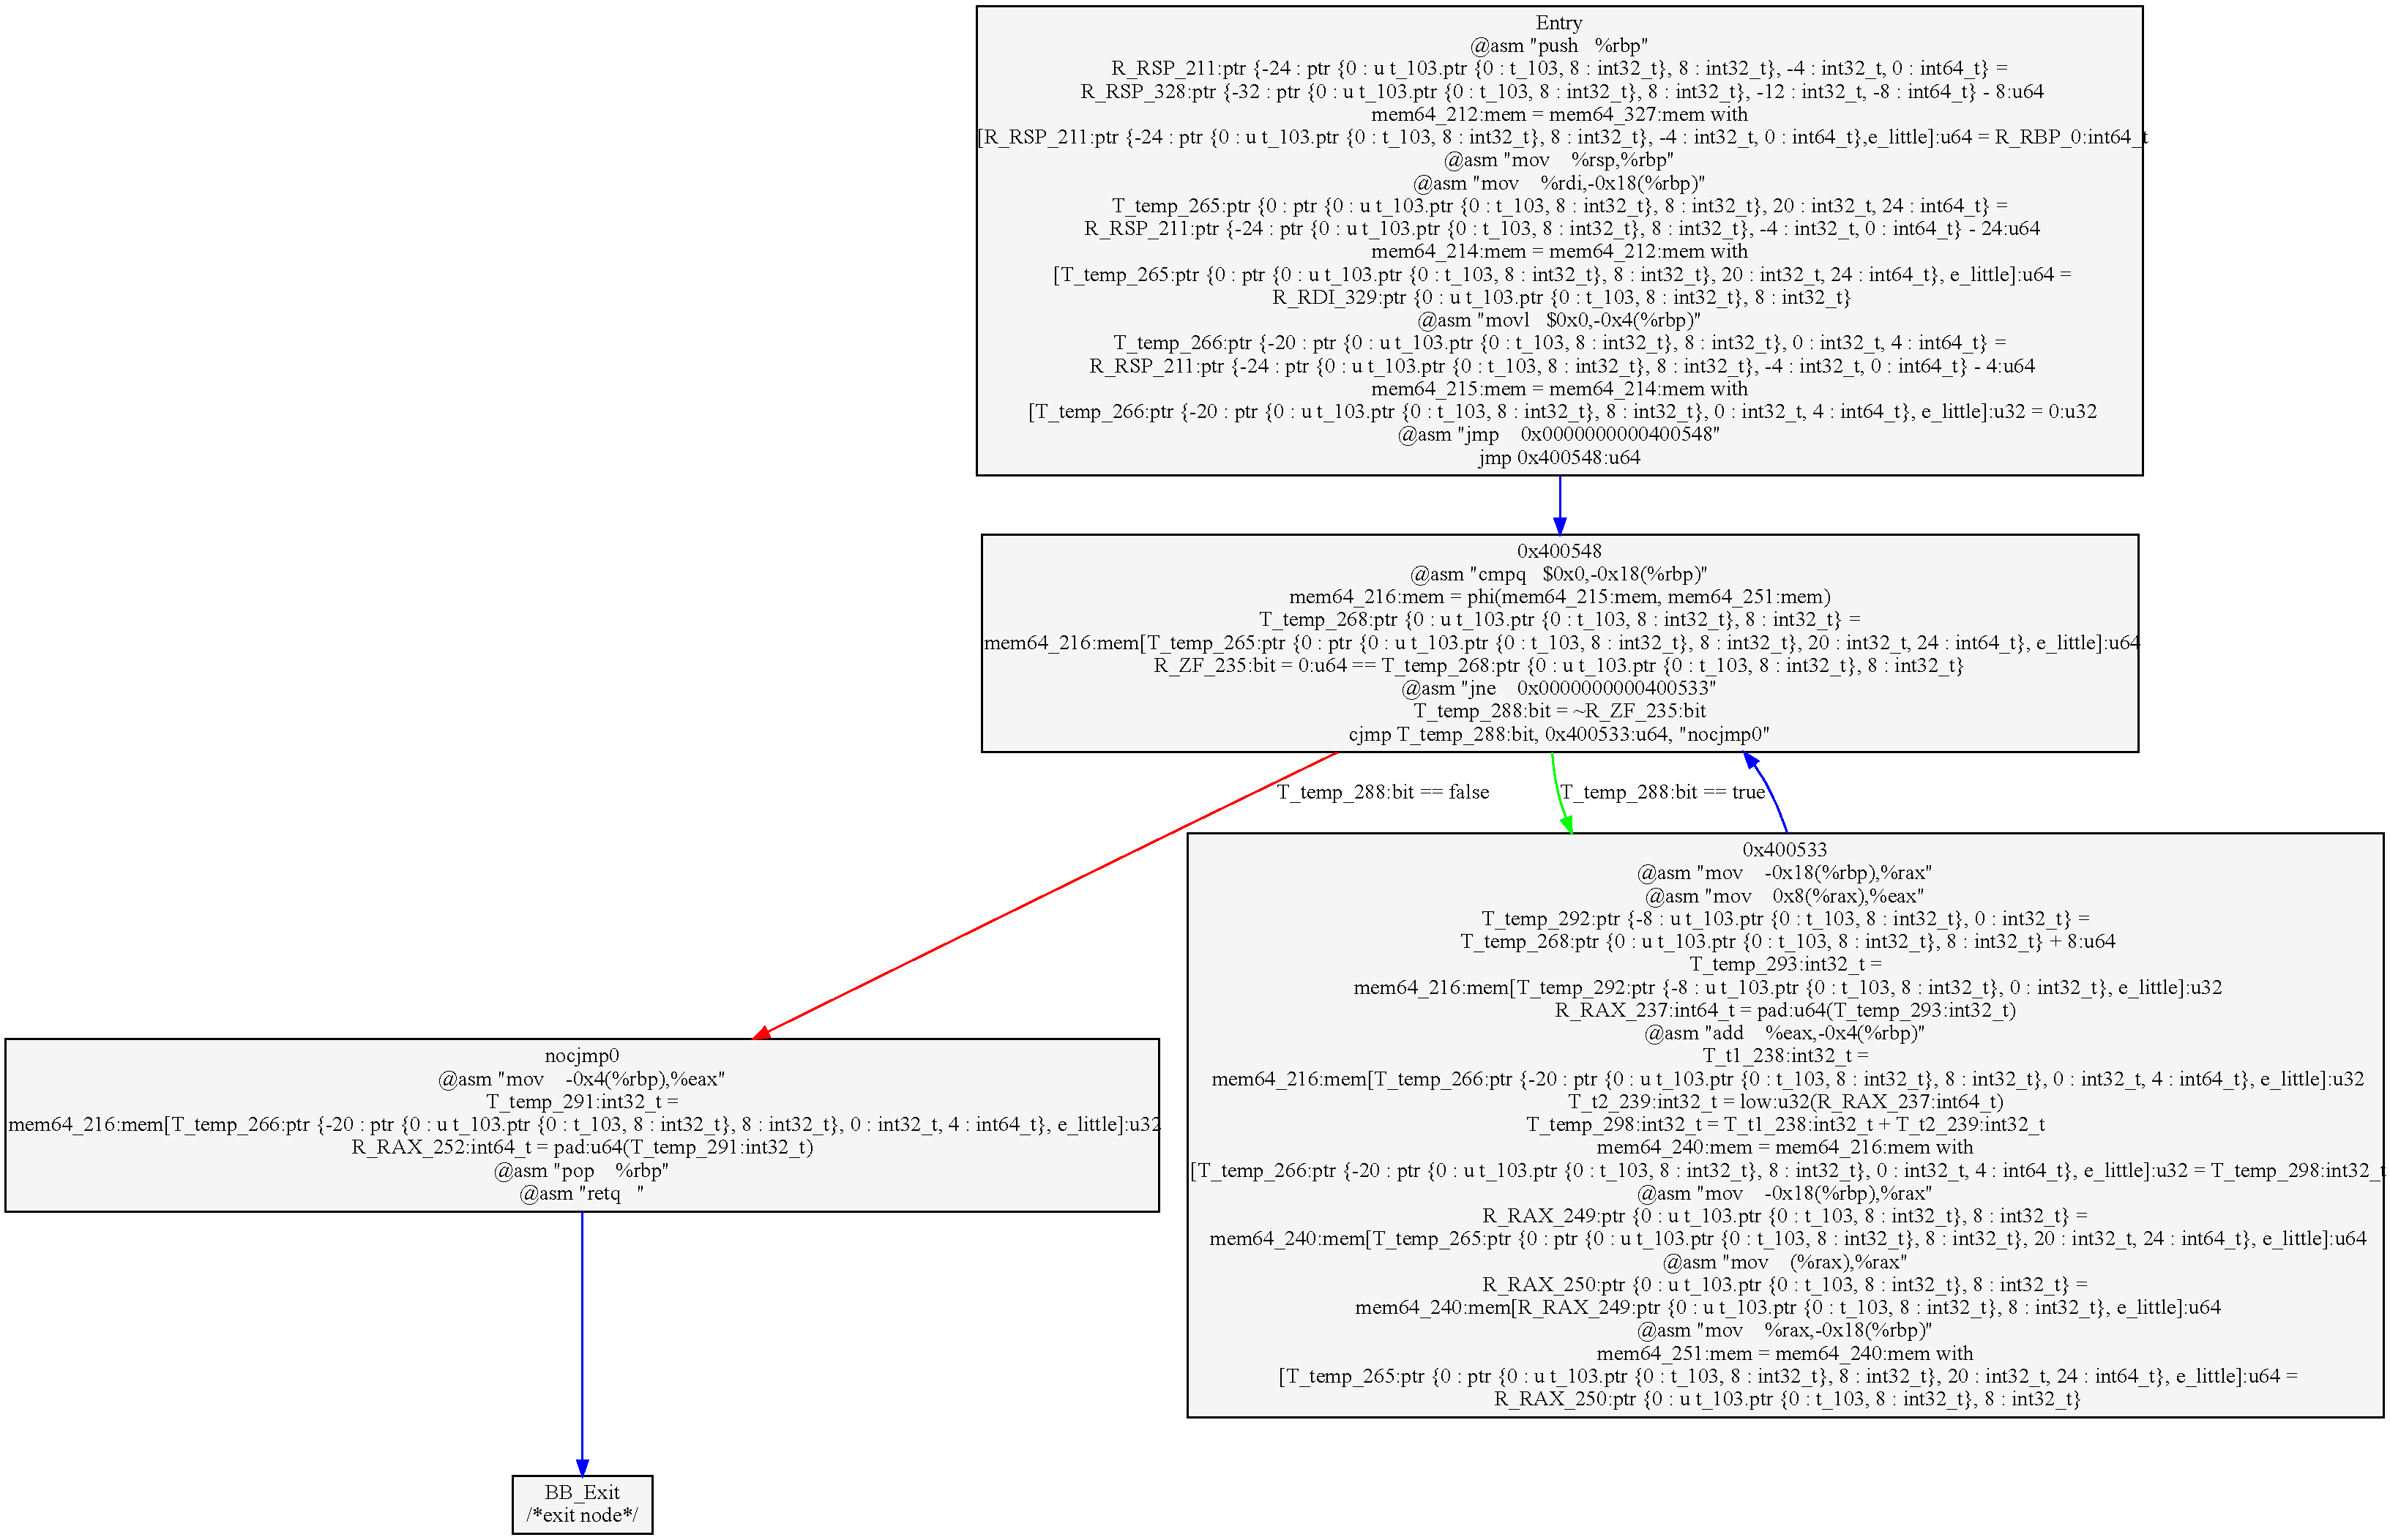
\includegraphics[scale=0.40,angle=90]{bitr/out2.pdf}
}
\caption{Solved List Summation}
\label{fig:solvedlist}
\end{figure*}

